\documentclass[12pt]{article}

\usepackage{amsbsy}
\usepackage{amsmath}
\usepackage[dutch]{babel}
\usepackage{graphicx}

% Stop indent in nieuwe paragraaf
\setlength\parindent{0pt}

\begin{document}
    
\title{\textbf{Practica BB1:} Viscositeit van vloeistoffen\\\small{groep 2\_5}}
\author{\textbf{Dries Van den Brande} \and Andreas Declreck \and Wassim Amghizar \and Joren Vermeesch}
\date{\today}

\maketitle

\section*{Verslagplan (verwijderen)}
\begin{itemize}
    \item Maak een verslag in Word (geen pdf?) en geen EXCEL in mail!
    \item Leg uit hoe je de metingen hebt uitgevoerd? welke problemen had je? hoe heb je deze opgelost
    \item Toon meetresultaten in grafiek en tabelvorm
    \item leg uit hoe je de berekeningen hebt uitgevoerd voor berekeningen van $\eta$
    \item leg uit hoe je de berekeningen hebt uitgevoerd voor de bepaling van de fout. Motiveer de methode
    \item Bespreek de resultaten
    \item Formuleer conclusies
\end{itemize}

\section{Doel van het practicum}

Svetlana.Verbruggen@vub.be

Emodulus bepalen
--> via rekstrookje, hoe werkt het?

Maat voor de stijheid van een materiaal. Sommige vervormen veel en andere weinig. Hoog weinig vervormen.

bpaling: door spanning = kracht / dwarsdoorsnele en wet van hooke

rekstrookje: kleine geleider, om de weerstand te bepalen. controle spanning op een materiaal.

Hoe werkt et: uitrek verandert de doorsnede --> verandering weerstan (pouillet)

basis eq: eq20
gausfactor: factor voor productiefouten

wat doen wij?
- Theoretisch berekenen van de gevoeligheid van beide types

opgave 2: schakeling maken, eerst paar dinge bereken (Theoretische waarde R en instellen)
welke combinatie mogen we niet maken?
bron niet meer ideaal --> 1.22
Interne weerstand verandert (hangt af van instelwaarde)

multimeter in gelijkstroon zetten

brug in evenwicht als Rmid = 0
dit door lineare interpolarisatie.

opgave 3: Emodulus bepalen

verslag:

Het doel van dit practicum wordt een brug van Wheatstone


\section{Doel}

In dit practicum wordt met behulp van de brug van Wheatstone
het elastisch gedrag van balkje met onbekende elasticitiet
onderzocht.


%\section{Theorie}

\subsection{Afleiding schuifkracht voor laminaire stroming en 
definitie van de viscositeit}

Als een voorwerp zich beweegt in een flu\"idum, dan verstoort het de snelheidsverdeling hiervan.
Vloeistofmoleculen die in onmiddelijk contact zijn met het voorwerp, krijgen door 
adhesiekrachten dezelfde snelheid, terwijl ver ervandaan het milieu niet verstoord wordt.\\

\begin{figure}[h]
    \centering
    \label{fig:snelheidsverdeling_laminair}
    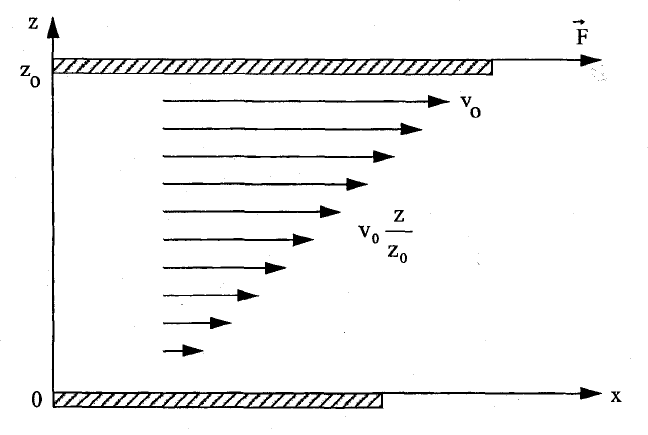
\includegraphics[width=0.7\textwidth]{img/figuur_1_theorie.png}
    \caption{Snelheidsverdeling in een viskeus midden tussen evenwijdige platen bij lage snelheden}
\end{figure}

Voor lage snelheden beweegt de vloeistof zich in lagen over elkaar. Dit heet \textbf{laminaire stroming}.
De laag $z = z_{0}$ heeft de snelheid $v_{0}$ de snelheid nul heeft. De snelheid van de 
vloeistoflagen daartussenin verandert lineair in functie van de hoogte z.
\\

$v = v_{0} \cdot \frac{z}{z_{0}}$ of $\frac{\delta v}{\delta z} = \frac{v_{0}}{z_{0}}$
\\

In het algemeen neemt de snelheid echter niet lineair toe met de dikte an de vloeistoflaag. 
De evenredigheidsconstante is ook afhankelijk van de aard van het flu\"idum, en wordt de
\textbf{viscositeitsco\"effici\"ent} genoemd. We bekomen de formule:
$$\frac{F_{W}}{S} = \eta \cdot \frac{dv}{dn}$$

Met
\\

$S=$ de oppervlakte van de vloeistoflagen

$n=$ de normaal loodrecht op dit oppervlak

$dv=$ de snelheidsverandering over de lengte

$dn=$ de normaal op S
\\

De \textbf{viscositeitsco\"effici\"ent} $\eta$ is dus de kracht per oppervlakte-eenheid nodig 
om snelheidsverschil van \'e\'en eenheid te handhaven tussen twee lagen vloeistof gelegen 
op een eenheidsfactor van elkaar.

\subsection{Laminaire stroming in een cilindervormige buis}

De wet van Hagen-Poiseuille geeft de snelheidsverdeling van de vloeistof 
in een horizontale cilindervormige buis bij stationaire, laminaire storming.
\\

$$v(r) = \frac{\pi(p_{1}-p_{2}) \cdot R^4}{4 \cdot L \cdot \eta}$$
\\
Het volumedebiet Q is het volume vloeistof dat per seconde door de buis stroomt.
Dit is te berekenen door die vergelijking over de doorsnede van de buis te integreren. 
Dit geeft: 
\\

$$\int_0^R2 \pi rdr \cdot v(r) = \frac{\pi(p_{1} - p_{2})\cdot R^4}{4 \cdot L \cdot \eta} $$
\\

Volgens de \textbf{wet van Poiseuille} is het debiet Q recht evenredig met het 
drukverschil $\delta p$ in het laminair regime. In een grafiek van Q in functie
van $\delta p$ geeft dit een rechte door de oorsprong; de richtingsco\"effici\"ent van de rechte is gelijk aan $\pi R^4 / 8\eta L$.
\\

\subsection{Overgang van laminair naar turbulent regime}

Als de snelheid echter te groot wordt, zal het laminair regime plaatsmaken voor een turbulent regime. 
Dit turbulente regime wordt gekenmerkt door wervelingen of draaikolkjes. Het hoogste
debiet waarbij de stroming nog juist stabiel laminair is, wordt het kritische debiet
$Q_{krit}$ genoemd.

\begin{figure}
    \caption{Grafiek overgang laminair naar turbulent regime}
    \label{fig:overgang_lam_turb}
    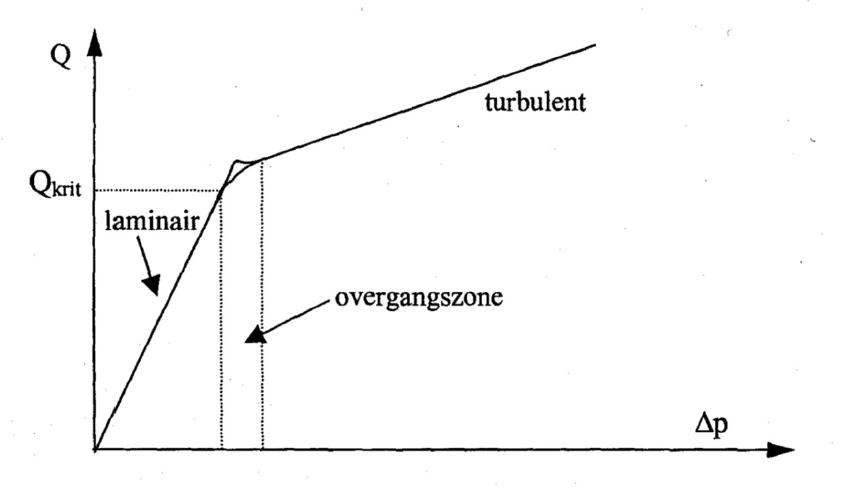
\includegraphics[width=0.7\textwidth]{img/figuur_3_theorie.png}
\end{figure}

Het is moeilijk om theoretisch te voorspellen bij welke stroomsnelheden laminaire
stroming zal overgaan in tubulente stroming. In dit kader speelt het 
\textbf{Reynoldgetal} een belangrijke rol.
\\

\subsection{Het Reynoldgetal}
De genormaliseerde gemiddelde stroomsnelheid $v/v_{0}$ wordt het Reynoldgetal genoemd:
\\

$$N_{R} = \frac{v \cdot \rho \cdot D}{\eta}$$
\\

Deze definitie geldt enkel voor een horizontale, cilindrische buis.
Voor andere systemen gelden andere definities.
\\

Het maximale Reynoldgetal waarbij de stroming nog juist stabiel is is ca. 2000.

\section{Methode}

Door middel van een Hagen-Poiseuille opstelling (Figuur \ref{fig:hagen-pois}), kunnen we
enkele versimpelingen bekomen.

\begin{figure}[h]
    \caption{Hagen-Poiseuille opstelling}
    \includegraphics[width=\textwidth]{img/hagen_poiseuille.png}
    \label{fig:hagen-pois}
\end{figure}


\section{Meetresultaten}

We hebben 16 metingen gedaan, waarvan 8 in het laminair regime en 
8 in het turbulent regime. Bij elke meting hebben we 3 keer de massa en
debiet gemeten.
\begin{center}
    \captionof{table}{Bekomen waarden voor het laminair regime}
    \begin{tabular}{| c | c | c | c | c |}
        \hline
        $\Delta h$ [m]  & $\Delta m$ [m]    & $\Delta t$ [s]    & $\Delta P$ [Pa]   & Q [$m^3$/s]      \\ \hline
        0,020           & 0,140             & 83,123            & 196,200           & 1,684E-06        \\ \hline
        0,026           & 0,138             & 78,613            & 255,060           & 1,760E-06         \\ \hline
        0,034           & 0,139             & 53,600            & 333,540           & 2,587E-06         \\ \hline
        0,054           & 0,143             & 42,963            & 529,740           & 3,334E-06         \\ \hline 
        0,060           & 0,138             & 35,097            & 588,600           & 3,941E-06         \\ \hline
        0,070           & 0,138             & 31,147            & 686,700           & 4,430E-06         \\ \hline
        0,092           & 0,138             & 24,480            & 902,520           & 5,637E-06         \\ \hline
        0,110           & 0,142             & 22,117            & 1079,100          & 6,424E-06         \\ \hline
    \end{tabular}
\end{center}
\begin{center}
    \captionof{table}{Bekomen waarden voor het turbulent regime}
    \begin{tabular}{| c | c | c | c | c |}
        \hline
        $\Delta h$ [m]  & $\Delta m$ [m]    & $\Delta t$ [s]    & $\Delta P$ [Pa]    & Q [$m^3$/s]      \\ \hline
        0,150           & 0,142             & 20,063            & 1471,500           & 7,064E-06        \\ \hline
        0,208           & 0,138             & 17,140            & 2040,480           & 8,072E-06         \\ \hline
        0,230           & 0,142             & 16,677            & 2256,300           & 8,495E-06         \\ \hline
        0,240           & 0,139             & 16,150            & 2353,400           & 8,627E-06         \\ \hline 
        0,246           & 0,138             & 15,787            & 2413,260           & 8,765E-06         \\ \hline
        0,280           & 0,141             & 15,253            & 2746,800           & 9,245E-06         \\ \hline
        0,350           & 0,142             & 13,420            & 3433,500           & 1,066E-05         \\ \hline
        0,434           & 0,142             & 11,800            & 4257,540           & 1,540E-05         \\ \hline
    \end{tabular}
\end{center}





\section{Berekening en fout viscociteitsconstante $\eta$}

De viscociteitsconstante in het laminaire regime is te berekenen aan de hand van de formule van Hagen-Poiseuille:
\begin{equation}
    \label{eq:hagen}
    Q = \frac{\pi \cdot \Delta P \cdot R^4}{8 \cdot L \cdot \eta}
\end{equation}
Deze formule is van de vorm $$y=a\cdot x$$ met de rico $a$ gelijk aan: $$a = \frac{\pi \cdot R^4}{8 \cdot L \cdot \eta}$$
Door middel van deze formule berekenen we $\eta$. \\

Deze $\eta$ zullen we bepalen door een lineaire regressie toe te passen op de gemeten waarden van het laminaire regime.
We bevinden ons in het geval van gelijkwaardige y-waarden.\\

Voor de lineaire regressie heb je het principe der kleinste kwadraten dat vereist
dat de $\chi ^2$-vorm minimaal is: 
\begin{equation}
    \chi ^2 = \sum\limits_{i=1}^n(y_i-a\cdot x_i)^2
\end{equation}
De beste schatting voor de richtingcoëfficiënt $a$ wordt gegeven door:
\begin{equation}
    \label{eq:a}
    \hat{a} \; \hat{=} \;\frac{\sum\limits_{i=0}^n x_i  y_i}{\sum\limits_{i=0}^n x_i^2}
\end{equation}
\begin{equation*}
    \hat{a} \; \hat{=} \; 6.31 \cdot 10^{-9}
\end{equation*}
Dus krijgen we de rechte: $$Q = 6.31\cdot 10^{-9} \cdot \Delta P$$

Hiermee kunnen we de $\chi ^2$-vorm bepalen:
\begin{equation*}
    \chi ^2 = 1.31 \cdot 10^{-10}
\end{equation*}
Door bepaling van de standaardafwijking: 
\begin{equation}
    \sigma ^2 = \frac{\chi ^2}{n - 1}
\end{equation}
\begin{equation*}
    \sigma ^2 = 1.88 \cdot 10^{-11}
\end{equation*}
kunnen we de betrouwbaarheid op de richtingscoëfficiënt $a$ berekenen: 
\begin{equation}
    \label{eq:sa}
    \sigma ^2 \{ a \} = \frac{\sigma ^2}{\sum\limits_{i=1}^n x_i^2}
\end{equation}
\begin{equation*}
    \sigma ^2 \{ a \} =  5.70 \cdot 10^{-18}
\end{equation*}
Waardoor we voor $a$ het volgend resultaat uitkomen:
$$a = 6.31 \cdot 10^{-9} \pm 5.70 \cdot 10^{-18}$$
Nu kunnen we uit formule \eqref{eq:hagen} viscociteitsconstante $\eta$ bepalen
\begin{equation*}
    \hat{\eta} = 9.89 \cdot 10^{-4}
\end{equation*}

Doordat $a$ een afschatting is en hiermee men de $\eta$ berekent,
moeten we ook de fout $\sigma ^2 \{ \eta \}$ bepalen

\begin{equation}
    \sigma ^2 \{ \eta \} = \left(\frac{\partial \hat{\eta}}{\partial \hat{a}}\right)^2 \cdot \sigma ^2 \{a\}
\end{equation}
\begin{equation*}
    \sigma ^2 \{ \eta \} = \left(\frac{\pi \cdot R^4}{8 \cdot L \cdot \hat{a^2}}\right)^2 \cdot \sigma ^2 \{a\}
\end{equation*}
Deze formule evalueren geeft ons:
\begin{equation*}
    \sigma \{ \eta \} = 1.40 \cdot 10^{-7}
\end{equation*}

met $a$ berekent in formule \eqref{eq:a} en $\sigma \{a\}$ in formule \eqref{eq:sa}

Ten slotte is de viscociteitsconstante gelijk aan:
\begin{equation*}
    \eta = (9.8909 \cdot 10^{-4} \pm 1.40 \cdot 10^{-7})Pa \cdot s
\end{equation*}\\

Nu kunnen we onze waarden in een grafiek gieten en krijgen we:
\begin{figure}[H]
    \centering
    \caption{Grafiek laminaire en turbulente stroom}
    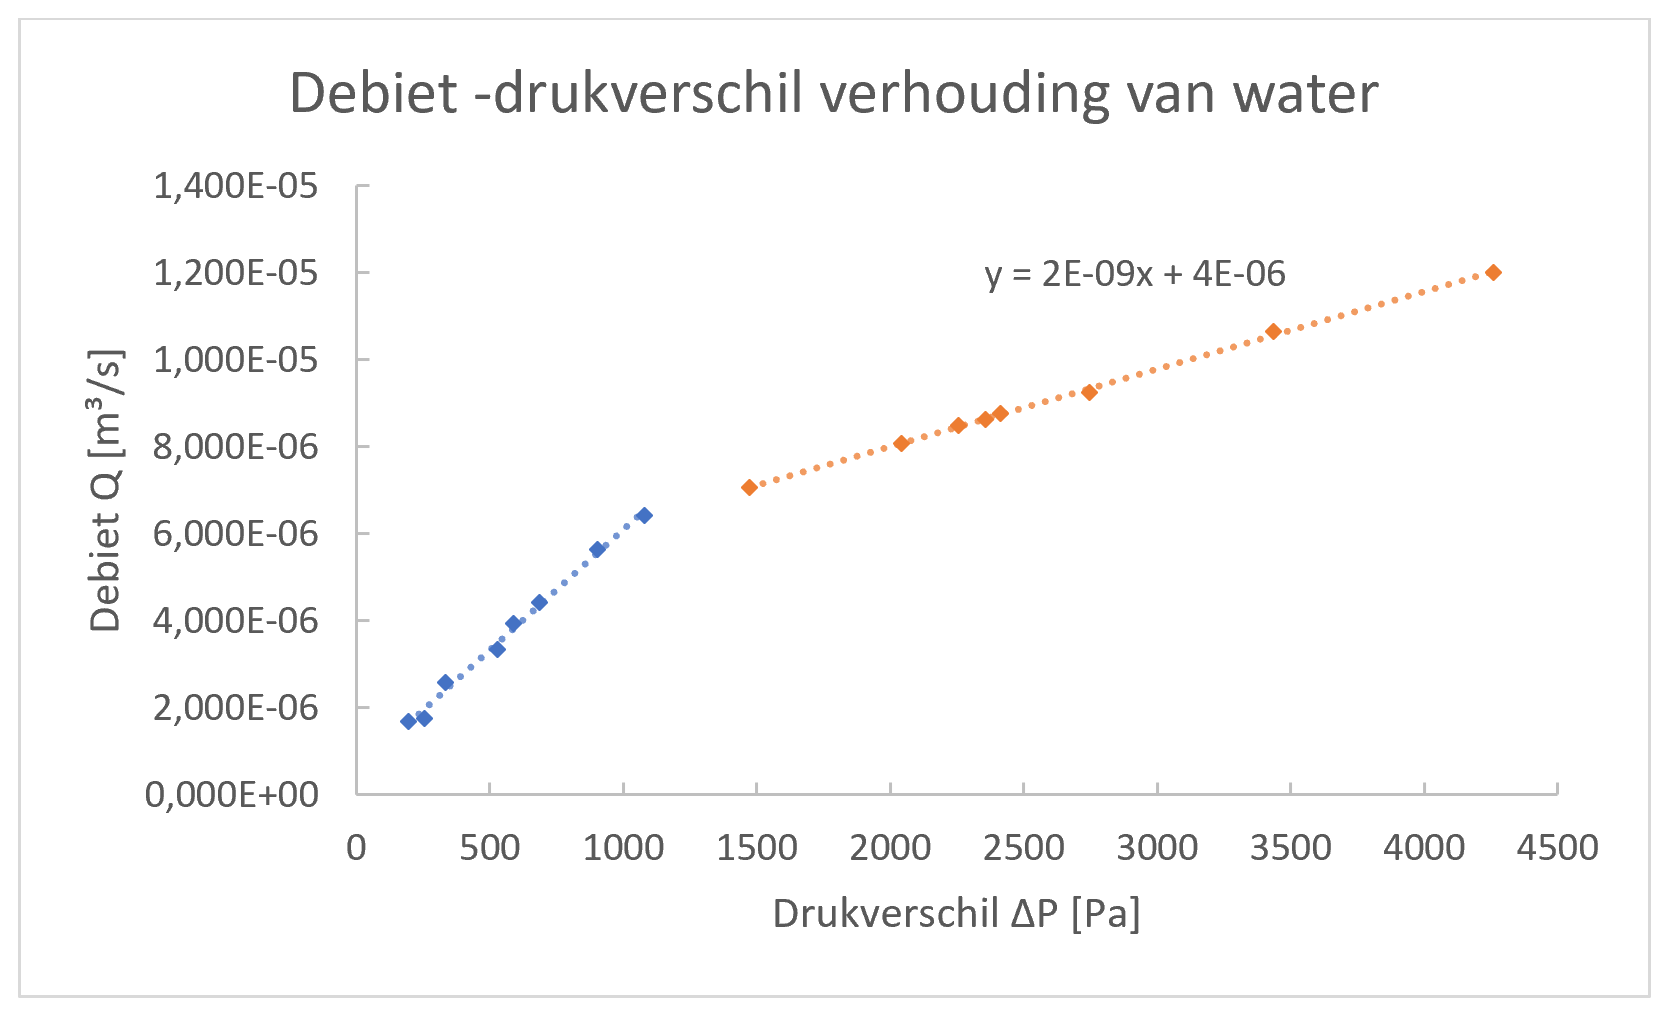
\includegraphics[width=0.8\textwidth]{img/grafiek.png}
    \label{fig:grafiek}
\end{figure}





\section{Berekening en fout Q$_{krit}$}

\section{Foutenanalyse}

\subsection{Rechtsteekse grootheden}

Te bespreken grootheden:
\begin{itemize}
    \item Verschil in hoogte $\Delta h$
    \item De massa $m$ van het opgevangen water
    \item Tijd $\Delta t$ nodig om beker te vullen
    \item Temperatuur $T$ van het water
\end{itemize}

\subsubsection{Systematische fouten}
Er bestaan 2 systematische fouten, namelijk afleesfouten en instrumentale fouten. Bij digitale meettoestellen wordt de afleesfout als $\pm 1$ eenheid genomen op het meest rechtse digit. 
Bij analoge toestellen daarentegen wordt de afleesfout als $\pm \frac{1}{2}$ van de kleinste schaalverdeling genomen. De instrumentale fout wordt berekend aan de hand van de door de producent gegeven rdg en dig. Aangezien we deze niet terugvinden hebben we de instrumentale niet kunnen bepalen.
\begin{itemize}
    \item $\Delta t$ werd gemeten aan de hand van een digitale chronometer. De afleesfout hierop bedraagt $\pm 0,01 s$.
    \item $m$ werd bepaald door middel van een digitale balans, de afleesfout is gelijk aan $\pm 1g$
    \item Aangezien $\Delta h$ verkregen werd door een relatieve meting uit te voeren, is de systematische fout gelijk aan 0. Hierdoor is de afleesfout te verwaarlozen.
    \item $T$ werd gemeten door middel van een analoge thermometer. De afleesfout is $\pm \frac{1}{2} \cdot 1C = \pm 0,5C$.
\end{itemize} 




\subsubsection{Toevallige fouten}
$\Delta T$ en $\Delta h$ werden telkens maar 1 maal gemeten, bijgevolg kan er niets gezegd worden over de toevallige fout op deze 2 grootheden.
\\
We bevinden ons in het geval gelijkwaardige grootheden aangezien deze telkens met hetzelfde meettoestel gemeten werden.
De toevallige fouten op $m$ en $\Delta t$ werden bepaald op basis van volgende formules:
\begin{equation}
    m = \frac{1}{n} \sum\limits_{i=1}^n x_i
\end{equation}

\begin{equation}
    \sigma^{2} \hat{=} \frac{\sum\limits_{i=1}^n (x_i - m)^2}{n - 1}
\end{equation} 

Voor $m$: \\
$m = $ %hier moet onze bepaalde waarde komen
$\Delta sigma^{2} = $ %hier moet onze bepaalde waarde komen 
\\
Voor $\Delta t$:\\
$m = $ %hier moet onze bepaalde waarde komen
$\Delta sigma^{2} = $ %hier moet onze bepaalde waarde komen



\subsection{Onrechtstreekse grootheden}

We berekenen het debiet $Q$ aan de hand van formule \eqref{eq:hagen}. Daarom is dit een onrechtstreeks gemeten grootheid.

Te bespreken grootheden:
\begin{itemize}
    \item Debiet $Q$
    \item Verschil in druk $\Delta p$
\end{itemize}

\subsubsection{Systematische fouten}
De systematische fout op $Q$ wordt berekend aan de hand van:
\begin{equation}
    \Delta Y = \sum\limits_{i=1}^n \left|\frac{\partial \Psi}{\partial x_i}\right|_o \cdot \Delta x_i
\end{equation}

\subsubsection{Toevallige fouten}



\section{Bespreking}

\section{Conclusie}
De berekende waarden zijn accuraat bepaald.
De schatting van het Reynoldgetal zou nog kunnen verbeterd worden door meer datapunten 
te meten rond het overgangspunt van laminair naar turbulent regime.

\bibliographystyle{plain}
\bibliography{../ref}

\begin{figure}[h]
    \centering
    \caption{Verband laminair/turbulent}
    \label{fig:verband_lam_turb}
    \setlength{\unitlength}{6cm}
    \begin{picture}(1.1, 1.1)
        \thinlines
        \put(0, 0){\vector(1, 0){1}}
        \put(0, 0){\vector(0, 1){1}}
        \thicklines
        \put(0, 0){\line(1, 3){0.1}}
        \put(0.1, 0.3){\line(1, 1){0.5}}
        \put(0.1, 0.3){\circle{0.05}}
        \put(0.01, 1){$Q$}
        \put(1, 0.01){$\Delta p$}
        \put(0.15, 0.25){$Q_{krit}$}
    \end{picture}
\end{figure}

\end{document}